\documentclass[12pt,titlepage]{article}
\usepackage{mathpazo}
\usepackage{color}
\usepackage[a4paper,lmargin={4cm},rmargin={2cm},tmargin={2.5cm},bmargin={2.5cm}]{geometry}
\usepackage[T1]{fontenc}
\usepackage[absolute,overlay]{textpos}
\usepackage[utf8]{inputenc}
\usepackage[ngerman]{babel}
\usepackage{blindtext}
\usepackage{graphicx}
\usepackage{wrapfig}
\usepackage{subfig}
\usepackage{multirow}
\usepackage{amsmath}
\usepackage{thmtools} 
\usepackage{amssymb} 
\usepackage{listings} 
\usepackage{siunitx}
\usepackage{tabularx}
\usepackage[pdfborder={0 0 0}]{hyperref}
\usepackage{breakurl}
\usepackage[onehalfspacing]{setspace}
\usepackage{cleveref}
\usepackage{smartdiagram}
\usepackage{placeins}
\lstset{numbers=left, numberstyle=\tiny, numbersep=5pt}
\lstset{language=Perl}

\begin{document}

\begin{titlepage}
\title{Crank-Nicolson-Methode}
\date{31.03.2022}
\author{Maurice Borries}
\maketitle
\end{titlepage}

\tableofcontents
\newpage
\section{Einleitung}
Ein wesentlicher Bestandteil des Finanzwesens ist es einen fairen Preis für Optionen zu finden. Der sogenannte Optionspreis ist der Preis, den der Käufer an den Halter einer Aktie bei Abschluss des Geschäftes zahlen muss. Um einen fairen Optionspreis berechnen zu können, müssen einige Aspekte berücksichtigt werden. Diese Ausarbeitung befasst sich mit der Berechnung eines europäischen Call-Preises nach Black-Scholes und der Finiten-Differenzen-Methode, die von John Crank und Phyllis Nicolson entwickelten Methode, der Crank-Nicholson-Methode. Hierzu wurde versucht ein Programm in Python zu entwickelt, dass die Crank-Nicholson-Methode selbstständig berechnet und diese veranschaulichen soll.
Bevor man allerdings genauer auf die Crank-Nicholson-Methode eingehen kann, müssen im Vorfeld einige grundlegende finanzmathematische Parameter erläutert werden. 
Um einen fairen Optionspreis berechnen zu können, müssen bestimmte Modellvoraussetzungen am Markt gelten. Es muss ein konstanter, risikoloser Zinssatz von 0 oder höher gelten $r\geq{0}$. Außerdem muss der Markt arbitragefrei sein und es darf keine Dividendenzahlungen auf den Aktienkurs geben. Ein arbitragefreier Markt bedeutet, dass man keine Möglichkeit hat einen Gewinn zu erzielen, ohne ein Risiko einzugehen. 
\\\\
\section{Unterschied zwischen Call und Put Optionen}
Bevor der Unterschied zwischen Call und Put Optionen genauer erklärt wird, muss im Vorfeld geklärt werden, was eine Option überhaupt ist. Eine Option gibt einem Käufer das Recht eine bestimmte Transaktion zu einem festgelegten Ausübungspreis, allerdings ist dies nicht verpflichtend, an bzw. bis zu einem bestimmten Zeitpunkt zu tätigen.
Eine Put-Option ist ein Vertrag zwischen zwei Parteien, die dem Käufer das Recht gibt, ein Wertpapier zu einem bestimmten Zeitpunkt zu einem im Vorfeld festgelegten Preis zu verkaufen.
Im weiteren Verlauf wird sich diese Ausarbeitung allerdings nur mit den Call-Optionen befassen.
Eine Call-Option ist ein Vertrag zwischen einem Käufer und einem Verkäufer, der dem Käufer das Recht gibt, ein Wertpapier zu einem festen Preis zu einem bestimmten Zeitpunkt zu erwerben.
Außerdem ist bei dem Call und Put Optionen auch zwischen der europäischen und amerikanischen Option zu differenzieren.
Die amerikanische Call-Option gibt dem Käufer das Recht, das Wertpapier zu dem festgelegten Preis zu jedem Zeitpunkt der Gesamtlaufzeit zu erwerben.
Bei der europäischen Call-Option ist dies nicht möglich, hier kann der Käufer das Wertpapier nur zu einem festgelegten Zeitpunkt kaufen.
\\\\
\section{Black-Scholes-Modell als Grundlage der Finiten Differenzenmethoden}
Das Black-Scholes-Modell ist eine Methode zur Bewertung von Optionen, die zum Ausübungszeitpunkt unendlich viele verschiedene Werte des Underyings besitzt. Unter Underyings zählen unter anderen Aktien ETF´s und Edelmetalle, die mit einem Optionsschein gezogen werden können. Um mit dem Black-Scholes-Modell verschiedene Optionen vergleichen zu können müssen die oben genannten Modellvoraussetzungen erfüllt sein und es muss sich außerdem um eine europäische Option handeln und es können Kredite in beliebiger Höhe können aufgenommen werden.
\\\\
Die Black-Scholes-Differenzialgleichung kann lediglich europäische Call und Put Optionen berechnen.\\
Black-Scholes-Differenzialgleichung\\
\begin{align*}
\frac{\partial V}{\partial t}+rS \frac{\partial V}{\partial S}+ \frac{1}{2} \sigma ^2 S^2 \frac{\partial ^2 V}{\partial S^2}=rV
\end{align*}\\
Mit Hilfe der Differenzialgleichung 
Black-Scholes-Modell und dem diskontierten Erwartungswert der Auszahlung ergibt sich die Preisformel. Auf eine Herleitung dieser Formel wird aufgrund des Umfanges dieser Ausarbeitung verzichtet.
\\
\begin{align*}
C=K*\Phi (d_1)-B*e^{-r_{k,f}+T}* \Phi (d_2)
\end{align*}
\\
Um die Bewertung eines Calls bestimmen zu können, müssen im Vorfeld einige Variablen festgelegt werden. Dies erfolgt am Beispiel der Salesforce Aktie (WKN: A0B87V). Der Kurspreis K sowie der Basiswert B werden mit 200€ festgelegt, dies entspricht in etwa den momentanen Preis der Aktie. Der risikofreie Zins $r_{k,f}$ ist fiktiv und wird mit 3\%  definiert. Außerdem muss die Laufzeit T festgelegt werden, in dem Folgenden Beispiel wird mit T=5 Jahre gerechnet. Die Volatilität liegt bei 53,8202\% , dies entspricht der Volatilität, die die Aktie in der 5 Jahreswertung hatte. Um diese Berechnung durchführen zu können, muss im zu Beginn $d_1$, sowie $d_2$ berechnet werden.\\\\
Die Formel für $d_1$ lautet: \\
\begin{align*}
d_1=\frac{ln(\frac{K}{B})+(r_{k,f}+\frac{\sigma{^2}_r}{2})*T}{\sigma _r *\sqrt{T}}
\end{align*}\\
Eingesetzt ergibt sich:\\
\begin{align*}
d_1&=\frac{ln(\frac{200}{200})+(0,03+\frac{0,538202^2}{2})*5}{0,538202 *\sqrt{5}}\\
d_1&=0,726369
\end{align*}\\
\\Diesen Wert muss man nun in der Verteilungsfunktion der Standartnormalverteilung suchen. Man erhält für den korrespondierenden Wert in der Verteilungsfunktion der Standartnormalverteilung 0,76730.
\\\\Um nun $d_2$ berechnen zu können muss man auf folgende Gleichung zurückgreifen:
\begin{align*}
d_2&=d_1-\sigma_r*\sqrt{T}\\
d_2&=0,726369-0,03+\sqrt{5}\\
d_2&=-0,4771
\end{align*}\\
Da man es nicht möglich ist, negative Zahlen aus der Verteilungsfunktion abzulesen, muss es hier nochmal zu einer Umformung kommen.\\
\begin{align*}
d_2&=1-\Phi (0,4771)\\
d_2&=1-0,68439    \\    
d_2&=0,31561
\end{align*}\\
Nun haben wir alle Variablen, um den Call bewerten zu können. Es entsteht folgende Gleichung:\\
\begin{align*}
C&=200Euro*0,76730-200Euro*e^{-0,03+5}*0,31561\\
C&=99,13Euro
\end{align*}
Der Wert des Calls beträgt zum Zeitpunkt t=0 also C=99,13€.
Da das Black-Scholes-Modell allerdings nur bei dem europäischen Put und Call Optionen anzuwenden ist, muss bei der Berechnung anderer Optionen wie z.B. der amerikanische Put und Call Option auf die Finite-Differenzen-Methoden zurückgegriffen werden. 
Hierbei ist bei den Finiten-Differenzen-Methoden zwischen drei Methoden zu differenzieren. Die implizierte Euler-Methode, die explizite Euler-Methode und die Crank-Nicolson-Methode.\\
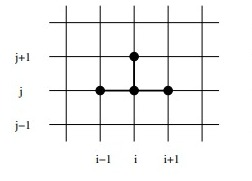
\includegraphics[width=5.8cm]{ex.png}  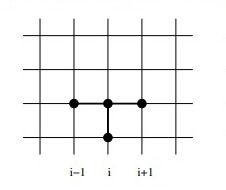
\includegraphics[width=5.3cm]{im.png} 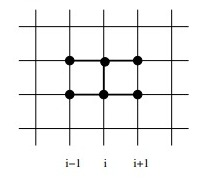
\includegraphics[width=4.9cm]{cn.png} \\\\
https://www.uni-frankfurt.de/53287938/blatt4.pdf\\
Bei der linken Grafik handelt es sich um eine Veranschaulichung der explizierten Euler-Methode, in der die Ableitung durch eine Vorwärtsdifferenz ersetzt wird. Bei der mittleren Grafik handelt es sich um die implizierte Euler-Methode, welche die Ableitung durch die Rückwartsdifferenz ersetzt. Im weiteren Verlauf wird allerdings lediglich die Crank-Nicolson-Methode weiter betrachtet.\\\\
Bei diese Methode wird die Differenzialquotienten des der Black- Scholes-\\Differenzialgleichung durch Differenzenquotienten vertauscht.  \\
\begin{align*}
\frac{\partial V}{\partial t}+rS \frac{\partial V}{\partial S}+ \frac{1}{2} \sigma ^2 S^2 \frac{\partial ^2 V}{\partial S^2}=rV
\end{align*}\\

\begin{align*}
\frac{\partial V}{\partial t}=v_t(t_i,S_j) & \approx \frac{V_{j,i+1}-V_{j,i}}{\triangle t}\\
\frac{\partial V}{\partial S}=v_s(t_i,S_j) & \approx \frac{V_{j+1,i+1}-V_{j-1,i+1}+V_{j+1,i}-V_{j-1,i}}{4 \triangle S}\\
\frac{\partial ^2 V}{\partial S^2}=v_ss(t_i,S_j) & \approx \frac{V_{j+1,i+1}-2V_{j,i+1}+V_{j-1,i+1}+V_{j+1,i}-2V_{j,i}+V_{j-1,1}}{2(\triangle S)^2}
\end{align*} \\
\\
Diese Approximation werden in die Black-Scholes-Differzialgleichung eingesetzt und es ergibt sich folgende Formel:\\\\
$-\frac{1}{4}rj \triangle t + \frac{1}{4} \sigma^2 j^2 \triangle  t V_{j-1,i}-1-\frac{1}{2}r \triangle t - \frac{1}{2} \sigma^2 j^2 \triangle t V_{j,i}+\frac{1}{4}rj \triangle t + \frac{1}{4} \sigma^2 j^2 \triangle  t V_{j+1,i}= -\frac{1}{4}rj \triangle t + \frac{1}{4} \sigma^2 j^2 \triangle  t V_{j-1,i+1}+\beta _j -1+\frac{1}{2}r \triangle t + \frac{1}{2} \sigma^2 j^2 \triangle  t V_{j,i+1}-\frac{1}{4}rj \triangle t + \frac{1}{4} \sigma^2 j^2 \triangle  t V_{j+1^,i+1}$ \\\\\\
Man definiert:\\\\
\begin{align*}
a_j&=-\frac{1}{4}rj \triangle t + \frac{1}{4} \sigma^2 j^2 \triangle  t\\
b_j&=-1-\frac{1}{2}r \triangle t - \frac{1}{2} \sigma^2 j^2 \triangle  t\\
c_j&=\frac{1}{4}rj \triangle t + \frac{1}{4} \sigma^2 j^2 \triangle  t\\
\beta _j&=-1+\frac{1}{2}r \triangle t + \frac{1}{2} \sigma^2 j^2 \triangle  t\\
\end{align*} \\\\
Dies hat zu Vorteil, dass die obrige Formel deutlich übersichtlicher aussieht und es ergibt sich folgende Formel:
\begin{align*}
a_jV_{j-1,i}+b_jV_{j,i}+c_jV_{j+1,i}=-a_jV_{j-1,i+1}+\beta _jV_{j,i+1}-c_jV_{j+1^,i+1}
\end{align*}\\
Aus dieser Gleichung lässt sich folgendes Matrix-System herleiten: \\\\
\begin{align*}
\begin{pmatrix}
b_1 & c_1 & 0 & \ldots & 0 & 0\\
a_2 & b_2 & c_2 & 0 & \ldots & 0\\
0   & a_3 & b_3 & c_3 & \ldots & 0\\
\ldots & \ldots & \ldots & \ldots& \ldots & 0\\
0 & \ldots & \ldots & \ldots & \ldots & \ldots
\end{pmatrix} \begin{pmatrix}
V_{1,i}\\
V_{2,i}\\
V_{3,i}\\
V_{4,i}\\
\ldots\\
\end{pmatrix} = \begin{pmatrix}
-a_1 V_{0,i+1}+\beta_1 V_{1,i+1}-c_1V_{2,i+1}-a_1V_{0,i}\\
-a_2 V_{1,i+1}+\beta_2 V_{2,i+1}-c_2V_{3,i+1}\\
-a_3 V_{2,i+1}+\beta_3 V_{3,i+1}-c_3V_{3,i+1}\\
\ldots\\
\ldots\\
\end{pmatrix}
\end{align*}
\\
Dieses Matrix-System muss dann mit Hilfe eines linearen Gleichungssystem gelöst werden, da dies allerdings einen enormen zeitlichen Aufwand bedeuten würde, wird dies mit Python automatisiert. Der R-Code hat mit den oben definierten Variablen folgenden Output geliefert.\\\\
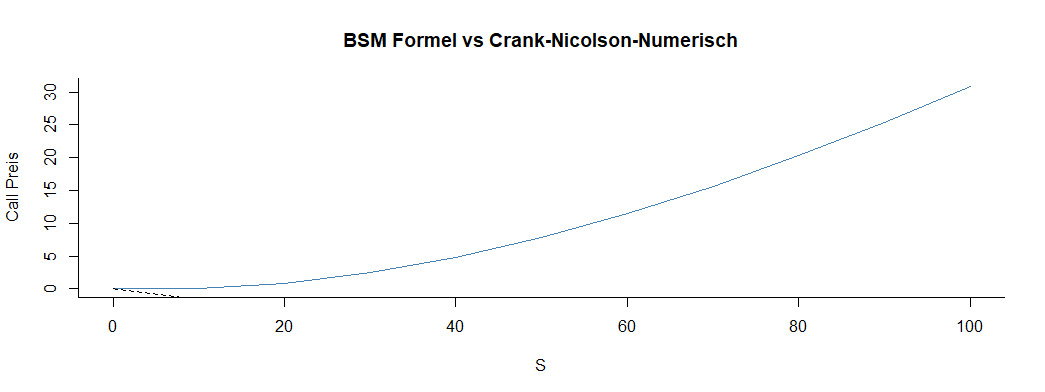
\includegraphics[width=15.3cm]{crank.png}
\\\\
\section{Programmierteil}
Nach zahlreichen Versuchen eine geeignete Lösung für die Crank-Nicolson-\\Methode in Python zu finden, musste ich  feststellen, dass all meine Versuche leider nicht zielführend waren und ich konnte auch keine andere alternative Lösung, die mir weiterhelfen konnte, online finden. Eine zweiwöchige Corona-\\Infektion hat mich zu dem zeitlich sehr weit nach hinten geworfen. Aus diesem Grund musste ich leider auf die von Ihnen zur Verfügung gestellte Lösung des Problems zurückgreifen und diese von R-Studo in Python implementieren. Leider war dies die einzige Möglichkeit, überhaupt eine Lösung präsentieren zu können.  \\\\
\section{Fazit}
Aufgrund der Problematik, die bei der Programmierung aufgetreten ist, war ein direkter Vergleich zwischen der Black-Scholes-Methode gegenüber der Crank-Nicolson-Methode nicht möglich. Die Methode handschriftlich zu lösen war durch die Komplexität des linearen Gleichungssystem leider nicht möglich.
\newpage
\section{Quellenverzeichnis}
\begin{itemize}
\item https://www.mathematik.tu-dortmund.de/papers/ThiemannAnstots\\KraftLiu GuoJoosten2014.pdf, Prof. Dr. Stefan Turek,
Dr. Thomas Hübner zuletzt abgerufen: 31.3.2022
\item https://moodle.htw-berlin.de/pluginfile.php/1357680/mod-resource/content/\\\\1/CompFiMa-VL5-komment-WS2022.pdf, Prof. Dr. Erlwein-Sayer, zuletzt abgerufen: 31.3.2022
\item https://dewiki.de/Lexikon/Crank-Nicolson-Verfahren zuletzt abgerufen: 29.3.2022
\item https://de.wikipedia.org/wiki/Finite-Differenzen-Methode zuletzt abgerufen: 27.3.2022
\item https://www.youtube.com/watch?v=lgEOBBNtjiI \\zuletzt abgerufen:20.3.2022
\item https://de.wikipedia.org/wiki/Crank-Nicolson-Verfahren zuletzt abgerufen: 22.3.2022
\item https://de.wikipedia.org/wiki/Standardnormalverteilungstabelle zuletzt abgerufen: 22.3.2022
\item https://studyflix.de/wirtschaft/black-scholes-modell-471 zuletzt abgerufen: 22.3.2022
\item http://webdoc.sub.gwdg.de/ebook/dissts/Koeln/Int-Veen2005.pdf zuletzt abgerufen: 23.3.2022
\item https://de.wikipedia.org/wiki/Black-Scholes-Modell\\ zuletzt abgerufen: 31.3.2022
\item https://www.math.uni-frankfurt.de/~harrach/lehre/Numerik-von\\ -Differentialgleichungen.pdf, Prof. Dr. Bastian von Harrach, zuletzt abgerufen: 31.3.2022, zuletzt abgerufen: 31.3.2022
\item https://moodle.htw-berlin.de/pluginfile.php/1354456/mod-resource/\\content/\\1/ImplicitBSPDGL\%20Eu\%20Call\%20Comp\%20Fin\%202021.R

\end{itemize}
\end{document}
